
%(BEGIN_QUESTION)
% Copyright 2006, Tony R. Kuphaldt, released under the Creative Commons Attribution License (v 1.0)
% This means you may do almost anything with this work of mine, so long as you give me proper credit

Given the liquid flowmeter and storage vessel shown here, determine the accumulated volume in the vessel at the following times, for the flow rates shown on the graph:

$$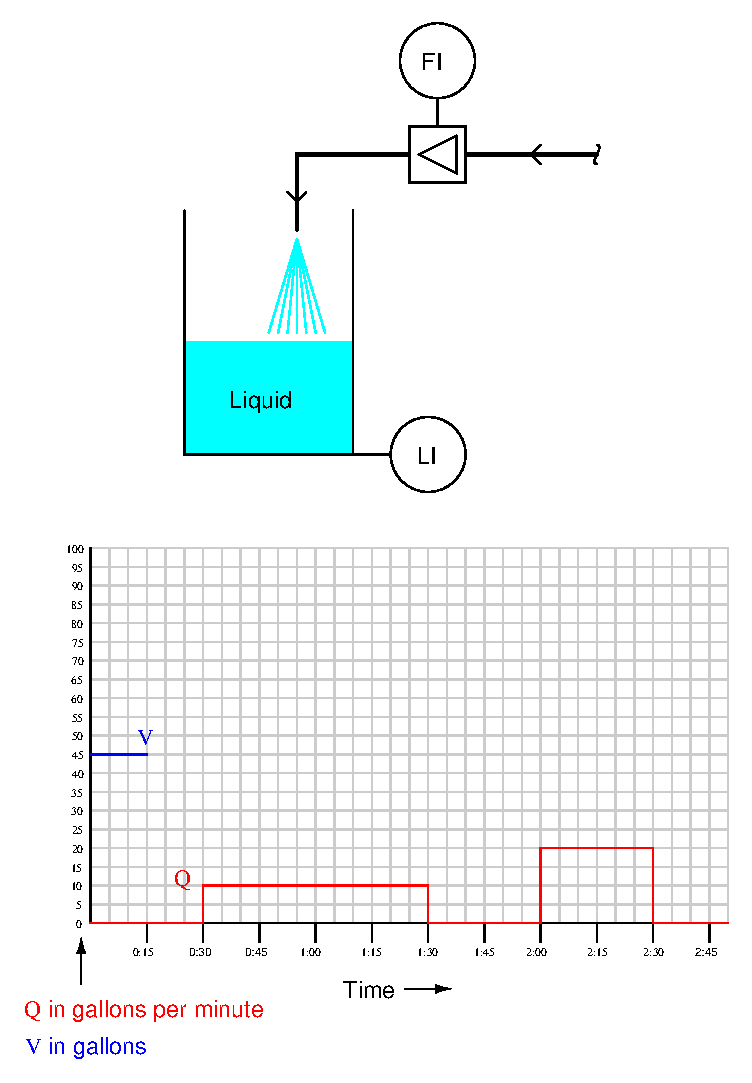
\includegraphics[width=15.5cm]{i01580x01.eps}$$

As indicated on the graph, the vessel holds 45 gallons of liquid at time = 0:00.  Note that the unit of time for the graph's horizontal axis is minutes:seconds, not hours:minutes.

\filbreak

\vskip 20pt \vbox{\hrule \hbox{\strut \vrule{} {\bf Suggestions for Socratic discussion} \vrule} \hrule}

\begin{itemize}
\item{} If you were standing in view of the pipe discharging water into this vessel, what would the liquid flow rate shown by the graph {\it look} like?  Would the flow vary over time, or would it remain steady?  Would it start and stop, or be continuous?
\item{} Suppose you were given a graph of water volume in the tank, and asked to calculate flow rate in or out of the tank.  What principle of calculus would you apply to solve this problem?
\item{} Suppose the flow rate ($Q$) shown on the graph represented flow {\it out} of the tank rather than flow {\it in} to the tank.  How would this difference affect the shape of the $V$ graph?
\item{} A tank being filled with water is analogous to an electrical capacitor being ``filled'' with charge.  Identify the appropriate variables for a graph showing the ``filling'' of a capacitor.
\end{itemize}

\underbar{file i01580}
%(END_QUESTION)





%(BEGIN_ANSWER)

$$\includegraphics[width=15.5cm]{i01580x02.eps}$$

%(END_ANSWER)





%(BEGIN_NOTES)

Up until time 0:30 the flow remains at 0 GPM.  Then, at 0:30 the flow increases to 10 GPM and holds steady at that rate until 1:30.  A flow rate of 10 GPM for a duration of 1 minute accumulates 10 gallons in the vessel, so during this time the volume steadily ramps from 45 gallons to 55 gallons.

\vskip 10pt

Then, at time 1:30 the flow ceases and remains at 0 GPM for 30 seconds.  At time 2:00 the flow resumes at a rate of 20 GPM, holding steady at that rate for 30 seconds.  A flow rate of 20 GPM for half a minute accumulates 10 gallons in the vessel, so the volume steadily ramps from 55 gallons to 65 gallons during that time.  Note how the same amount of volume accumulation takes place in half the time as before (between 0:30 and 1:30), due to the doubled flow rate (20 GPM instead of 10 GPM).

\vskip 10pt

At time 2:30 the flow ceases again and remains at 0 GPM for the remainder of the graph's horizontal axis.  Thus, the vessel volume holds constant (flat line) at 65 gallons.





\vskip 20pt \vbox{\hrule \hbox{\strut \vrule{} {\bf Suggestions for Socratic discussion} \vrule} \hrule}

\begin{itemize}
\item{} Propose a different flow trend recording to students (e.g. different duration, different magnitude) and have them predict the resulting alteration of the volume trend.
\item{} Propose a different volume trend recording to students and have them predict the necessary flow trend profile to cause it.
\end{itemize}

%INDEX% Mathematics, calculus: integral (accumulated volume as the integral of flow)

%(END_NOTES)


